\documentclass[11pt,
  paper=a4, 
  bibliography=totocnumbered,
	captions=tableheading,
	BCOR=10mm
]{scrreprt}

\usepackage[utf8]{inputenc}
 
 
\usepackage[onehalfspacing]{setspace}
\usepackage{csquotes} % Context sensitive quotation.
\usepackage{amsmath} % Standard math.
\usepackage{amsthm} % Math theorems.
\usepackage{amssymb} % More math symbols.
\theoremstyle{definition}
\newtheorem{definition}{Definition}[chapter]
 
\usepackage[section]{placeins} % Keep floats in the section they were defined in.
\usepackage{tabularx}
\usepackage{booktabs} % Scientific table styling.
\usepackage{floatrow} % Option for keeping floats in the place they were defined in the code.
\floatsetup[table]{style=plaintop}
\usepackage{hyperref} % Hyperlinks.
\usepackage[all]{nowidow} % Prevent widows and orphans.
\usepackage{xstring} % logic string operations
\usepackage[nopostdot, nonumberlist]{glossaries} % glossary for definitions and acronyms, without dot after entry and page reference 
\usepackage{bbm} % \mathbb on numerals.
\usepackage{csquotes}
\usepackage{mathtools}
\usepackage[ruled,vlined]{algorithm2e} % Pseudocode
\usepackage{scrhack} % Make warning go away.
\usepackage{graphicx}
\usepackage{subcaption} % Subfigures with subcaptions.
\usepackage{authoraftertitle} % Make author, etc., available after \maketitle
\usepackage{listofitems}
\usepackage{blindtext} % Placeholder text.
\usepackage[nopostdot, nonumberlist]{glossaries}
\makeglossaries % Generate the glossary

% \PassOptionsToPackage{obeyspaces}{url}%
\usepackage[backend=bibtex,% 
style=nature,% 
doi=true,isbn=false,url=false, eprint=false]{biblatex}
% \renewbibmacro*{url}{\printfield{urlraw}}

\addbibresource{bib/library.bib}

\DeclareStyleSourcemap{
  \maps[datatype=bibtex, overwrite=true]{
    \map{
      \step[fieldsource=url, final]
      \step[typesource=misc, typetarget=online]
    }
    \map{
      \step[typesource=misc, typetarget=patent, final]
      \step[fieldsource=institution, final]
      \step[fieldset=holder, origfieldval]
    }
  }
}

%\linespread{1.5} % set line spacing
 
\usepackage{listings} % rendering program code
\lstset{% general command to set parameter(s)
	basicstyle=\ttfamily\color{grey},          % print whole listing small
	keywordstyle=\color{black}\bfseries\underbar,
	% underlined bold black keywords
	identifierstyle=,           % nothing happens
	commentstyle=\color{white}, % white comments
	stringstyle=\ttfamily,      % typewriter type for strings
	showstringspaces=false}     % no special string spaces


\DeclareFontFamily{U}{mathx}{\hyphenchar\font45}
\DeclareFontShape{U}{mathx}{m}{n}{
      <5> <6> <7> <8> <9> <10>
      <10.95> <12> <14.4> <17.28> <20.74> <24.88>
      mathx10
      }{}
\DeclareSymbolFont{mathx}{U}{mathx}{m}{n}
\DeclareFontSubstitution{U}{mathx}{m}{n}
\DeclareMathSymbol{\bigtimes}{1}{mathx}{"91}

 

%%% Custom definitions %%%
% Shorthands
\newcommand{\ie}{i.\,e.~}
\newcommand{\eg}{e.\,g.~}
\newcommand{\ind}{\mathbbm{1}}
% Functions
\newcommand{\tpow}[1]{\cdot 10^{#1}}
\newcommand{\figref}[1]{(Figure \ref{#1})}
\newcommand{\figureref}[1]{Figure \ref{#1}}
\newcommand{\tabref}[1]{(Table \ref{#1})}
\newcommand{\tableref}[1]{Table \ref{#1}}
\newcommand{\secref}[1]{%
	\IfBeginWith{#1}{chap:}{%
		(cf. Chapter \ref{#1})}%
		{(cf. Section \ref{#1})}%
		}
\newcommand{\sectionref}[1]{%
	\IfBeginWith{#1}{chap:}{%
		Chapter \ref{#1}}%
		{\IfBeginWith{#1}{s}{%
			Section \ref{#1}}%
			{[\PackageError{sectionref}{Undefined option to sectionref: #1}{}]}}}
\newcommand{\chapref}[1]{(see chapter \ref{#1})}
\newcommand{\unit}[1]{\,\mathrm{#1}}
\newcommand{\unitfrac}[2]{\,\mathrm{\frac{#1}{#2}}}
\newcommand{\codeil}[1]{\lstinline{#1}}{} % wrapper for preventing syntax highlight error
\newcommand{\techil}[1]{\texttt{#1}}
\newcommand{\Set}[2]{%
  \{\, #1 \mid #2 \, \}%
}
% Line for signature.
\newcommand{\namesigdate}[1][5cm]{%
	\vspace{5cm}
	{\setlength{\parindent}{0cm}
	\begin{minipage}{0.3\textwidth}
		\hrule 
		\vspace{0.5cm}
		{\small city, date}
	\end{minipage}
	 \hfill
	\begin{minipage}{0.3\textwidth}
		\hrule
		\vspace{0.5cm}
	    {\small signature}
	\end{minipage}
	}
}
% Automatically use the first sentence in a caption as the short caption.
\newcommand\slcaption[1]{\setsepchar{.}\readlist*\pdots{#1}\caption[{\pdots[1].}]{#1}}

% Variables. 
% Adapt if necessary, use to refer to figures and graphics.
\def \figwidth {0.9\linewidth}
\graphicspath{ {./graphics/figures/}{./graphics/figures/} } % Path to figures and images.


% Customizations of existing commands.
\renewcommand{\vec}[1]{\mathbf{#1}}
% Capitalized \autoref names.
\renewcommand*{\chapterautorefname}{Chapter}
\renewcommand*{\sectionautorefname}{Section}


% TODO Fill with your data.
\title{My full title}
\author{Sven Groen}

\begin{document}

\begin{titlepage}
	\begin{flushleft}
		Universität Osnabrück\\
		Fachbereich Humanwissenschaften\\
		Institute of Cognitive Science
	\end{flushleft}

	\vspace{2cm}
	\centering{
		Bachelorthesis\vspace{1cm}\\
		\textbf{\Large{\MyTitle}}
		\vspace{1cm}\\
		\begin{tabular}{c}
			\MyAuthor                          \\
			970219                            \\
			Bachelor's Program Cognitive Science \\
			Starting month and year - end month and year
		\end{tabular}}
	\vspace{1cm}

	\begin{tabular}{ll}
		First supervisor:  & Dr. Ulf Krumnack          \\
		                   & Institute of Cognitive Science            \\
		                   & Osnabrück                \\\\
		Second supervisor: & Manuel Kolmet         \\
		                   & IMANOX GmbH  \\
		                   & Berlin 
	\end{tabular}

\end{titlepage}


\chapter*{Declaration of Authorship}
I hereby certify that the work presented here is, to the best of my knowledge and belief, original and the result of my own investigations, except as acknowledged, and has not been submitted, either in part or whole, for a degree at this or any other university.

\namesigdate
\pagenumbering{gobble}
\pagebreak

\begin{abstract}
	\textbf{\LARGE{Abstract}}\\\\
	%TODO summarize the main objectives and outcomes of your work. The abstract should fit on one page.
	This is the abstract.
\end{abstract}




%\tableofcontents
%\listoffigures
%\listoftables
%\listofalgorithms


\chapter{Introduction}
\pagenumbering{arabic}
\section{Motivation}
- usually flickering between two frames of the video sequence, 
and ghost objects or partly incorrectly segmented objects often occur only in a single frame, 
while they are classified correctly in the next frame.\cite{Pfeuffer2_2019}

\section{Goal of the thesis}
\section{Semantic Segmentation}
\section{Recurrent Neural Networks}

Recurrent Neural Networks (RNNs) are a special kind of artificial neural network that is able to process sequential data \cite{Valipour2017, Sherstinsky2020} and "extract temporal dependencies" \cite{Hochreiter1998}.
In Sequential data the order of the data is of importance and therefore carries information, for example speech recognition or time variant problems \cite{Hoffmann2017, Pfeuffer2_2019}.
RNNs contain a hidden recurrent state, which enables them to process sequential data \cite{Hoffmann2017, Valipour2017}.
Although they have been applied succesfully to many problems in the sequential data domain \cite{Sherstinsky2020}, they are often criticized for their computational complexity due to their recurrent structure \cite{Pfeuffer2_2019}.
They are also known for struggling in learning long term dependencies \cite{Hoffmann2017}.

The reason for this is the vanishing- and exploding gradient effect \cite{Hochreiter1998}.
\textcite{Hochreiter1991} was the first to identified the vanishing gradient effect \cite{Skansi2018}.
The gradient of the loss is used to update the models weights during the backpropagation, enabling the "learning" of the model \cite{Suzuki2017, Skansi2018}.
The gradient of early layers of deep networks dependent on the gradient of later layers, since the gradient is propagated backwards through the network \cite{Skansi2018}.
For recurrent neural networks this backpropagation of the gradient is called \textit{backpropagation through time} (BPTT) \figref{fig:rnn-bptt-with-gradients}, 
where the gradient for any time step is dependent on all previous timesteps \cite{Skansi2018}.


\begin{figure}[H]
	\centering
	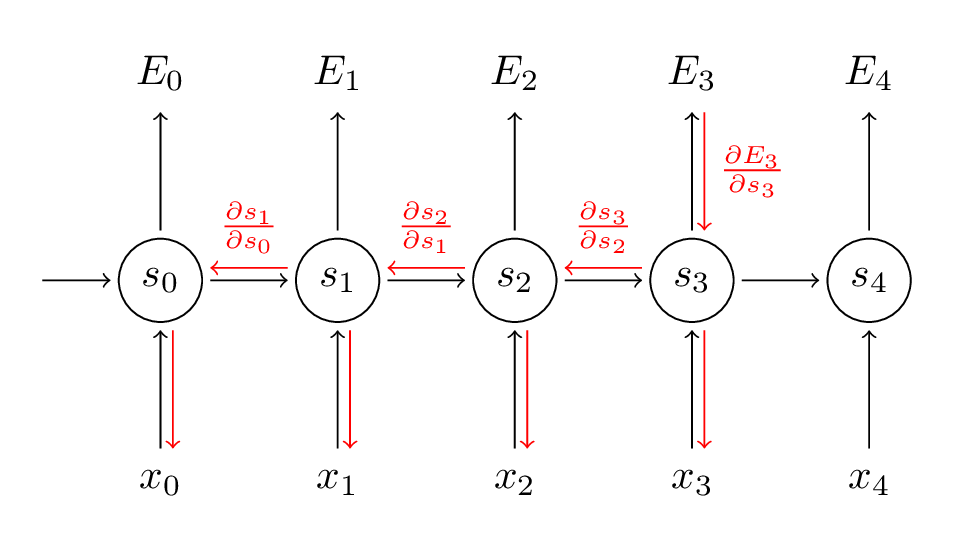
\includegraphics[width=\figwidth]{rnn-bptt-with-gradients}
	\slcaption{
		Backpropagatiob through time (\textcite{Britz2015}).
		\label{fig:rnn-bptt-with-gradients}}
\end{figure}

The \textit{vanishing gradient effect} occurs since derivatives are repeatedly multiplied \cite{Skansi2018}. 
If a gradient is zero or close to zero the amount of learning in the previous layers is very small, 
since their gradient is very small due to their predecessors being very small \cite{Britz2015, Hochreiter1991}.
\textcite{Pascanu2013} states that the \textit{vanishing gradient effect} occurs 
"when long term components go exponentially fast to norm 0, 
making it impossible for the model to learn correlation between temporally distant events."

During an explosion of long term dependencies the \textit{exploding gradient effect} occurs \cite{Pascanu2013}.
Here, during backpropagation the gradient can can grow exponentially with each layer \cite{Philipp2017, Hochreiter1997}.
The \textit{learning step} would simply be to large, leading us not closer to an optimum but further away \cite{Skansi2018}.



\subsection{LSTM}
- can be categorized as subgroup of rnn \cite{Hoffmann2017}


LSTM structure;
- gates control back propagation flow between each node; \cite{Valipour2017}
- These gates can learn the optimal way to remember useful information from previous states and decide the current state. \cite{Valipour2017}


convLSTM;
- In contrast to the conventional LSTMs that use fully connected layers in the input-to-state and state-to-state transitions, ConvLSTM uses convolutional layers instead. \cite{Nabavi2018}
- Their advantage is that they are translational invariant analogously to convolution layers and the required model parameters can be significantly reduced \cite{Pfeuffer2_2019}
- They use convolutional layers in their input-to-state and state-to-state transitions instead of fully connected layers, as conventional LSTMs [8] do. \cite{Pfeuffer2_2019}
- \cite{Pfeuffer2_2019} introduced different versions of the conv LSTMs



\subsection{GRU}
GRU structure + difference to LSTM;
- simpler Architecture -> faster + less memory consuming \cite{Valipour2017}
- "LSTM updates its hidden state by summation over flow after input gate and forget gate.
   GRU however, assumes a correlation between how much to keep from the current state and 
   how much to get from the previous state and it models this with the zt gate." \cite{Valipour2017}


convGRU;

\section{Related Work}
\chapter{Methods}
\section{The Dataset}
\section{Preprocessing}
\section{Network Architecture}
\section{Training}
\chapter{Results}
\chapter{Evaluation and Discussion}
\chapter{Conclusion}


\chapter*{Acknowledgements}
%TODO A place to say thank you to everybody who helped you.


% Acronym definitions
%TODO Add acronym definitions produced by acronyms2glossary.py 




\glsaddall
\printglossaries

\printbibliography

\end{document}